\documentclass[a4paper, 11pt]{article}
\usepackage[a4paper, left=3cm, right=2cm, top=2cm]{geometry}
\usepackage[utf8]{inputenc}					% Zeichenkodierung UTF-8 falls Probleme wegen utf8 auftreten, utf8 durch utf8x ersetzen
\usepackage[ngerman]{babel}					% Deutsche Sprache und Silbentrennung
\usepackage{xcolor}
\usepackage{amsmath}						% erlaubt mathematische Formeln
\usepackage{amssymb}						% Verschiedene Symbole
\usepackage{graphicx}						% Zum Bilder einfügen benötigt
\usepackage{hyperref}						% Sprunglinks für Überschriften, Fußnoten und Weblinks
\usepackage{tabularx}
\usepackage{siunitx}                        % Zur Darstellung von SI Einheiten
\sisetup{
  locale = DE ,
  per-mode = symbol
}
\usepackage{multicol}                       % Mehrspaltig

\usepackage{parskip}                        % No Space after newline

\newcommand\mainformular[1]{\fbox{#1}}      % Standard Formel
\newcommand\legende[1]{
    \colorbox{lightblue}{%
    \begin{tabularx}{\textwidth}{llll}
     #1
    \end{tabularx}
    }
}                                           % Farbig hintelegte Legende
\definecolor{lightblue}{RGB}{204, 230, 255}

\begin{document}

\section{Messtechnik}

\subsection{Grundlagen Drehspulmesser}
\subsubsection{Windungen im Wickelraum}
\begin{minipage}{0.45\textwidth} 
\mainformular{ $A_W = N \cdot d^2$} \\
\end{minipage} 
\begin{minipage}{0.45\textwidth} 
 
\legende{ 
$A_W$ & Wickelraum & & \\
$N$ & Anzahl der Windungen &  & \\
$d^2$ & Drahtdurchmesser & \si{\square\metre} & \\
} 
\end{minipage}

\subsubsection{Elektrisches Moment} 
\begin{minipage}{0.45\textwidth} 
\mainformular{ $M_{el}= A \cdot N \cdot B \cdot I$} \\
\end{minipage} 
\begin{minipage}{0.45\textwidth} 
 
\legende{ 
$N$ & Anzahl der Windungen &  & \\
$I$ & Stromstärke & \si{\ampere} & \\
$A$ & Fläche & \si{\square\metre}  & \\
$B$ & Feldstärke & \si{\tesla} & \\
} 
\end{minipage}

\subsubsection{Mechanisches Moment} 
\begin{minipage}{0.45\textwidth} 
\mainformular{ $M_{mech}= \alpha \cdot D$} \\
\end{minipage} 
\begin{minipage}{0.45\textwidth} 
\legende{ 
$D$ & Federkonstante & $\si{\newton\metre}/90\si{\degree}$ & \\
$\alpha$ & Ausschlagwinkel & \si{\degree} & \\
} 
\end{minipage}

\subsubsection{Zeigerausschlag}
\begin{minipage}{0.45\textwidth}
\mainformular{ $\alpha = I \cdot \cfrac{A\cdot N\cdot B}{D}$}
\end{minipage}
\begin{minipage}{0.45\textwidth}
\legende{
$N$ & Anzahl der Windungen &  & \\
$I$ & Stromstärke & \si{\ampere} & \\
$A$ & Fläche & \si{\square\metre}  & \\
$D$ & Federkonstante & \si{\newton\metre} & \\
}
\end{minipage}

\subsubsection{Strommessung mit Nebenwiderstand}
\begin{minipage}{0.45\textwidth}
\mainformular{ $(I-I_M) R_N= I_M(R_M+R_V)$ }\\
$R_N = \cfrac{I_M(R_M+R_V)}{I-I_M} $
\end{minipage}
\begin{minipage}{0.45\textwidth}
\legende{
$I_M$ & Messwerkstrom & \si{\ampere} &  \\
& 1\si{\milli\ampere} oder 100\si{\micro\ampere} & & \\
$I$ & Stromstärke & \si{\ampere} & \\
$R_M$ & Spulenwiederstand (Kupfer*) & \si{\ohm}  & \\
$R_N$ &  & \si{\ohm} & \\
$R_V$ &  & \si{\ohm} & \\
}
*Temperaturkoeffizient Kupfer: $4\%/10\si{\kelvin}$
\end{minipage}


\subsubsection{Güteklasse mit Temperaturkoeffizient} 
\begin{minipage}{0.45\textwidth} 
\mainformular{ $G = \cfrac{R_M}{R_M+R_V}\cdot 4\%/10 \si{\kelvin}$ } \\
\end{minipage} 
\begin{minipage}{0.45\textwidth} 
 
\legende{ 
$G$ & Güteklasse & & \\
$R_M$ & Spulenwiederstand (Kupfer*) & \si{\ohm}  & \\
$R_N$ &  & \si{\ohm} & \\
$R_V$ &  & \si{\ohm} & \\
} 
\end{minipage}

\subsubsection{Rückwirkungsfehler Strommessung} 
\begin{minipage}{0.45\textwidth} 
\mainformular{ $F_I = \cfrac{I_M - I_0}{I_0} = -\cfrac{R_M}{R_0 + R_L + R_M}$ } \\
\end{minipage} 
\begin{minipage}{0.45\textwidth}  
\legende{ 
$F_I$ & systemischer Fehler & & \\
$I_0$ & &  \si{\ampere} & \\
$I_M$ & &  \si{\ampere} & \\
$R_0$ & &  \si{\ohm} & \\
$R_L$ & Lastwiderstand & \si{\ohm} & \\
$R_M$ & Spulenwiederstand (Kupfer*) & \si{\ohm}  & \\
} 
\end{minipage}

\subsubsection{Spannungsmesser} 
\begin{minipage}{0.45\textwidth} 
\mainformular{ $R_V = \cfrac{U}{I_M} - R_M$ } \\
\end{minipage} 
\begin{minipage}{0.45\textwidth}  
\legende{ 
$I_M$ & &  \si{\ampere} & \\
$R_M$ & Spulenwiederstand (Kupfer*) & \si{\ohm}  & \\
$R_V$ & Vorwiderstand & \si{\ohm} & \\
$U$ & Spannung & \si{\volt} & \\
} 
\end{minipage}

\subsubsection{Rückwirkungsfehler Spannungsmessung} 
\begin{minipage}{0.45\textwidth} 
\mainformular{ $F_U = \cfrac{U_M - U_0}{U_0} = -\cfrac{R_0}{R_0 + R_i}$ } \\
$U_M = \cfrac{U_0}{R_0+R_i}R_i$ \\
$R_i = R_M + R_V$
\end{minipage} 
\begin{minipage}{0.45\textwidth}  
\legende{ 
$F_U$ & systemischer Fehler & & \\
$U_0$ & &  \si{\volt} & \\
$U_M$ & &  \si{\volt} & \\
$R_0$ & &  \si{\ohm} & \\
$R_i$ & & \si{\ohm} & \\
$R_M$ & Spulenwiederstand (Kupfer*) & \si{\ohm}  & \\
$R_V$ & Vorwiderstand & \si{\ohm} & \\
} 
\end{minipage}


\subsection{Grundlagen DVN}
\subsubsection{DVN Genauigkeit Bit}
\begin{minipage}{0.45\textwidth}
\mainformular{ $B(n) = \cfrac{\log(2\cdot 10^n)}{\log(2)}$}
\end{minipage}
\begin{minipage}{0.45\textwidth}
\legende{
$n$ & Stellen der Anzeige & $\mathbb{N}$ & \\
}
\end{minipage}

\subsubsection{DVN Genauigkeit \%} 
\begin{minipage}{0.45\textwidth} 
\mainformular{ $e_r= \cfrac{1}{2 \cdot 10^n - 1}$} \\
$e_r= \cfrac{1}{2^{B(n)} - 1}$
\end{minipage} 
\begin{minipage}{0.45\textwidth} 
 
\legende{ 
$n$ & Stellen der Anzeige & $\mathbb{N}$ &  \\ 
 \\ 
} 
\end{minipage} 

\subsubsection{Anzeigen Auflösung} 

Bestimmung durch den Kehrwert der Anzeige. Beispiel für $3\frac{1}{2}$ 

\begin{minipage}{0.45\textwidth} 
\mainformular{ $0.5 \cdot 10^{-3}$} \\
\end{minipage} 
\begin{minipage}{0.45\textwidth} 
\end{minipage} 

\subsubsection{Spannung pro Digit} 
\begin{minipage}{0.45\textwidth} 
\mainformular{ $I_{Dig} = I \cdot n$} \\
\end{minipage} 
\begin{minipage}{0.45\textwidth} 
 
\legende{ 
$n$ & Kehrwert der Anzeige &  &  \\ 
$Mess_{max}$ & Max Wert Messbereich &  & \\
} 
\end{minipage} 

\subsubsection{Rückwirkungsfehler} 
Dieser ist größer als bei Analogen Messverfahren denn $R_P \ge R_M$.

\begin{minipage}{0.45\textwidth} 
\mainformular{ $F_I = \cfrac{I_M - I_0}{I_0} = -\cfrac{R_P}{R_0 + R_L + R_P}$ } \\
\end{minipage} 
\begin{minipage}{0.45\textwidth} 
 
\legende{ 
$F_I$ & systemischer Fehler & & \\
$I_0$ & &  \si{\ampere} & \\
$I_M$ & &  \si{\ampere} & \\
$R_0$ & &  \si{\ohm} & \\
$R_L$ & Lastwiderstand & \si{\ohm} & \\
$R_P$ & & \si{\ohm}  & \\
} 
\end{minipage}

\subsubsection{Rückwirkungsfehler Spannungsmessung} 
\begin{minipage}{0.45\textwidth} 
\mainformular{ $F_U = \cfrac{\cfrac{R_i R_P}{R_i + R_P}-R_P}{R_P} = -\cfrac{R_P}{R_i + R_P}$ } \\
\end{minipage} 
\begin{minipage}{0.45\textwidth} 
 
\legende{ 
$F_U$ & systemischer Fehler & & \\
$U_0$ & &  \si{\volt} & \\
$U_M$ & &  \si{\volt} & \\
$R_0$ & &  \si{\ohm} & \\
$R_i$ &  & \si{\ohm} & \\
$R_M$ & Spulenwiederstand (Kupfer*) & \si{\ohm}  & \\
$R_V$ & Vorwiderstand & \si{\ohm} & \\
} 
\end{minipage}


\section{Regelungstechnik}
\subsection{Stabilität von Regelkreisen}
Es gilt:

\begin{minipage}{0.45\textwidth}

\mainformular{ $F_G = \frac{F_o}{1 + F_o}$} \\
\mainformular{ $F_G = \frac{Z_o}{Z_o + N_o}$} \\
\mainformular{ $F_o = F_R \cdot F_S$} \\

\end{minipage}
\begin{minipage}{0.45\textwidth}

\legende{
$F_G$ & geschlossener Kreis  & & \\
$Z_o$ & Zähler offener Kreis  & & \\
$N_o$ & Nenner offener Kreis  & & \\
$F_o$ & offener Kreis  & & \\
$F_G$ & geschlossener Kreis  & & \\

}
\end{minipage}

\subsubsection{Hurwitz-Kriterium}
charakteristische Gleichung des geschl. Regelkreises:
$$ a_mp^m + a_{m-1}p^{m-1}+ ... + a_1p+ a_0 = 0$$

notwendige Bedingung: alle Koeffizienten der charakteristischen Gleichung des geschlossenen Regelkreises müssen vorhanden und positives Vorzeichen haben. \\

hinreichende Bedingung: Alle Hauptabschnitssdeterminanten $D_i$
der Hurwitzdeterminantte H müssen positiven Wert haben.\\

\begin{minipage}{0.45\textwidth}

\mainformular{ $D_2 = a_1\cdot a_2 - a_3 \cdot a_0$} \\
\end{minipage}
\begin{minipage}{0.45\textwidth}

\legende{
$D_2$ & Determinante rel. für System 3.Ord.  & & \\

}
\end{minipage}

\subsubsection{Niquist-Kriterium}
Der geschlossene Regelkreis ist stabil, wenn der kritische Punkt (-1,0) links der Ortskurve $F_o(j\omega)$ seines offenen Kreises liegt.

\begin{minipage}{0.45\textwidth}

\mainformular{ $F_o(j\omega) = \frac{K}{A(j\omega)+ j B(j\omega)}$} \\
$\omega_k \Rightarrow B(\omega) = 0$ \\
$\frac{K}{A(\omega_k)} > -1 $
\end{minipage}
\begin{minipage}{0.45\textwidth}

\legende{
$F_o(j\omega)$ & Übertragungsfkt. offenen Kreis  & & \\
& Berechnungen zum Prüfen d. Stabilität & & \\
}
\end{minipage}


\subsection{Regelgüte}
\begin{minipage}{0.45\textwidth}
$F_z(p) = \frac{x(p)}{Z(p)} = \frac{-F_s}{1+F_o} = 0$ \\
 $F_W(p) = \frac{x(p)}{w(p)} = \frac{F_o}{1+F_o} = 1$ \\

\end{minipage}
\begin{minipage}{0.45\textwidth}

\legende{
$F_z(p)$ & ideales Störverhalten  & & \\
$F_W(p)$ & ideales Führungsverhalten &  & \\
}
\end{minipage}

\subsubsection{Bleibende Regelabweichung Führungsverhalten}
\begin{minipage}{0.45\textwidth}
\mainformular{ $R_{1W} = \lim \limits_{p \rightarrow 0} \frac{1}{1+F_o(p)}$} \\
$R_{1WP} = \frac{1}{1+V_o}$ \\
 $R_{1WI} = 0$ \\

\end{minipage}
\begin{minipage}{0.45\textwidth}

\legende{
$R_{1W}$ & bleibende Regelabweichung  & & \\
& Führungsverhalten allgemein & & \\
$R_{1WP}$ & P-Regelkreis (ohne I-Glied) & & \\
$R_{1WI}$ & I-Regelkreis  & & \\

}
\end{minipage}

\subsubsection{Bleibende Regelabweichung Störverhalten}
\begin{minipage}{0.45\textwidth}
\mainformular{ $R_{1Z} = \lim \limits_{p \to 0} \frac{F_s(p)}{1+F_o(p)}$} \\
 $R_{1ZP} = \lim \limits_{p \to 0} \frac{F_s}{1+F_RF_S} = \frac{V_S}{1+V_RV_S} \approx \frac{1}{V_R}$ \\
$R_{1ZIS} = \lim \limits_{p \to 0} \frac{1}{pT_{IS}+ V_R} = \frac{1}{V_R}$ \\

\mainformular{ $R_{1ZIR} = \lim \limits_{p \to 0} \frac{pT_{IR}* V_S}{pT_{IR}+ V_S} = 0$} \\

\end{minipage}
\begin{minipage}{0.45\textwidth}

\legende{
$R_{1Z}$ & bleibende Regelabweichung  & & \\
& Störverhalten allgemein & & \\
$R_{1ZP}$ & P-Regelkreis (ohne I-Glied)  &  & \\
& für $V_RV_S >> 1$ & & \\
$R_{1ZIS}$ & I-Regelkreis, Strecke mit I-Glied  & & \\
$R_{1ZIR}$ & I-Regelkreis, Strecke ohne I-Glied  & & \\

}
\end{minipage}

\subsubsection{Geschwindigkeitsfehler}
Führungsgröße als Rampenfunktion \\
$ w(t) = a\cdot t \Rightarrow w(p) = \frac{a}{p^2}$\\

\begin{minipage}{0.45\textwidth}
\mainformular{ $R_{2} = \lim \limits_{p \to 0} p \cdot w(p) \frac{1}{1+F_o(p)}= 
\lim \limits_{p \to 0}  \frac{a}{p} \cdot \frac{1}{1+F_o(p)}$}  \\
$R_{2P} = \lim \limits_{p \to 0}  \frac{a}{p} \cdot \frac{1}{1+V_o}= \infty$\\
$ R_{2I} = \frac{aT_o}{V_o}$\\

\end{minipage}
\begin{minipage}{0.45\textwidth}

\legende{
$R_{2}$ & Geschwindigkeitsfehler  & & \\
&  allgemein & & \\
$R_{2P}$ & P-Regelkreis (ohne I-Glied)  &  & \\
$R_{2I}$ & I-Regelkreis  & & \\

}
\end{minipage}


\subsection{Optimierung einschl Regelkreise}
\begin{itemize}
  \item Strukturoptimierung
  \item Parameteroptimierung
  \item Verifikation
\end{itemize}
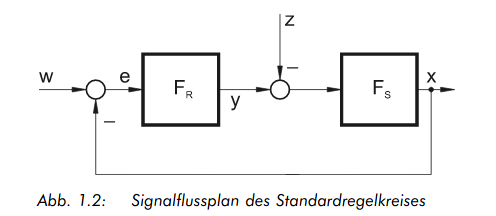
\includegraphics[scale= 0.5]{themen/pict/standardregelkreis.png}

\subsubsection{Enstellregel nach Ziegler/Nichols}
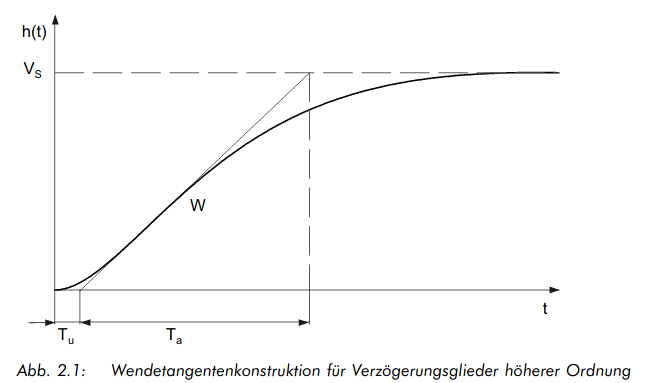
\includegraphics[scale= 0.5]{themen/pict/wendetangente.png}

Zur Messung an der Stabilitätsgrenze sind folgende Schritte nötig:\\
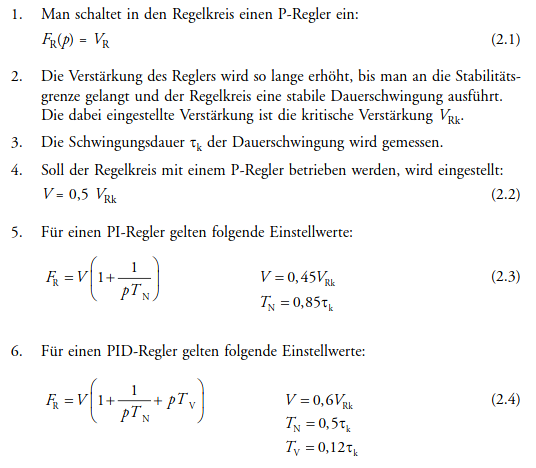
\includegraphics[scale= 0.5]{themen/pict/variante1-ziegler.png}

Wenn die Messung an der Stabilitätsgrenze nich möglich ist, wird die Sprungantwort gemessen. \\
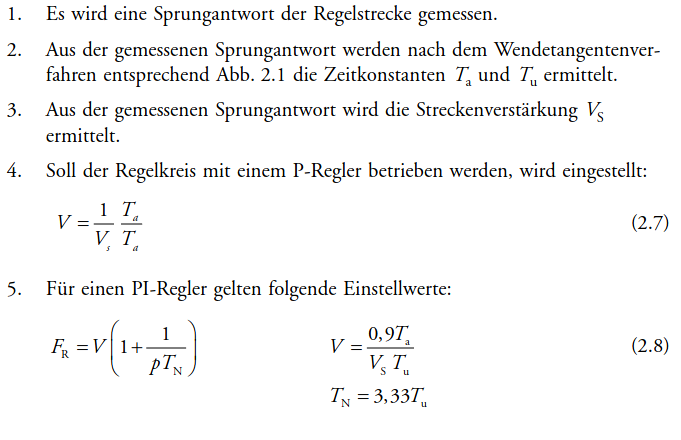
\includegraphics[scale= 0.5]{themen/pict/variante2.png}\\
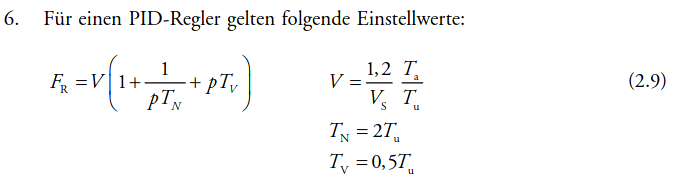
\includegraphics[scale= 0.5]{themen/pict/variante2-2.png}

\subsubsection{Einstellregel nach Chien/Hrones/Reswick}
unterscheidet zwischen Einstellung nach optimalem Führungsverhalten oder Störverhalten, jeweils ohne und mit $20\%$ Überschwingung.

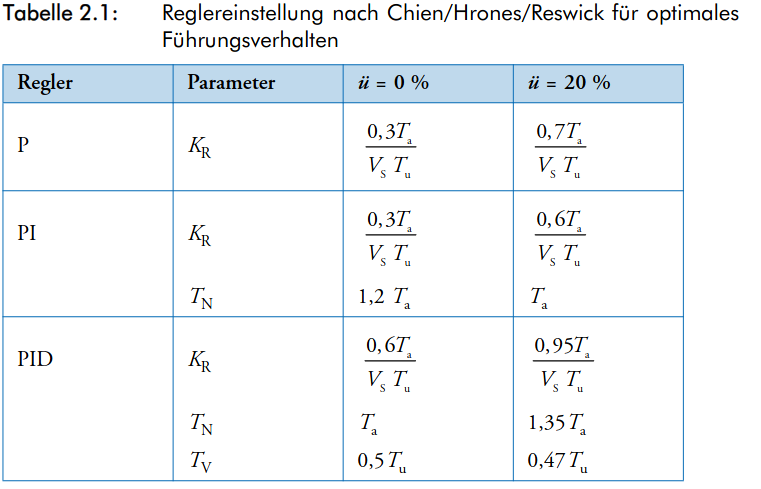
\includegraphics[scale= 0.5]{themen/pict/chien-fuehrung.png}\\

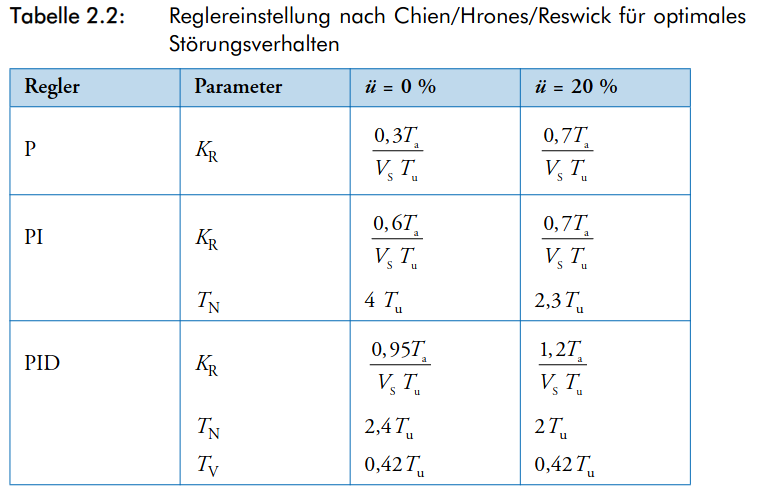
\includegraphics[scale= 0.5]{themen/pict/chien-stoerung.png}

Einstellwerte sind für ideale PID-Regler. Um sie realisierbar zu machen braucht es noch ein Verzögerungsglied.
Zeitkonstante $T_d = 3 \dots 50 T_v$. Experimentell bestimmt, beginnend bei $T_d = 4 T_v$

\subsubsection{Quadratisches Optimum }

 \begin{minipage}{0.45\textwidth}
  $\frac{dISE_3}{dV} = \frac{1}{2}\frac{a(bV - cV^2)-(aV+b)(b-2cV)}{(bV-cV^2)^2} = 0 $ \\
 $ V^2 + 2\cdot \frac{b}{a}\cdot V - \frac{b^2}{ac} = 0$
 aufgeläst ergibt sich:
 $ T_0 = V_s \cdot \frac{(T_1+T_2)\sqrt{T_1T_2}+T_1T_2}{T_1+T_2}$


 Mit zusätzlichem Verzögerungsglied wird Führungsverhalten verbessert (weniger Überschwingen)\\
 $F_V(p) = \frac{1}{1+pT_V} $ \\
 mit $T_{VQO} = 1,2 T_{\Sigma}$
 \end{minipage}
 \begin{minipage}{0.45\textwidth}

\legende{Ziel: Quadratische Regelfläche ISE wird \\minimal, allerdings großer Rechenaufwand\\}
 \legende{

 $\frac{dISE_3}{dV}$ & Ableitung  nach V  & & \\

 }
 \end{minipage}

\subsubsection{Betragsoptimum}
\begin{minipage}{0.45\textwidth}

vereinfachte Regelstrecke\\
$F_s = \frac{V_s}{\prod_{i=1}^k (1+pT_i)(1+pT_{\Sigma})}$\\
PID-Regler:\\
$F_R=\frac{\prod_{s=1}^r(1+pT_{RS})}{pT_0}$\\
offener Kreis ist damit:\\
$ F_0 = \frac{V_s \cdot \prod_{s=1}^r(1+pT_{RS})}{\prod_{i=1}^k (1+pT_i)(1+pT_{\Sigma})\cdot pT_0  }$
\end{minipage}
\begin{minipage}{0.45\textwidth}

\legende{
einfache, übersichtliche Einstellregeln\\ für Standardregelkreis\\

geeignet zur Ausregelung von Störgrößen,\\ die am Ausgang der Regelstrecke angreifen.


}
\end{minipage}


\textbf{Schritte zum Betragsoptimum:} \\
\begin{enumerate}
  \item Anzahl der Zählerzeitkonstanten des Reglers ist gleid der Anzahl k der großen Zeitkonstanten der Regelstrecke.
  \item Je eine Zählerzeitkonstante des REglers sei einer der großen Zeitkonstaten der Strecke gleich. $T_{Rs} = T_i $
  \item Einstellregel für die Integrierzeitkonstante:\\
  $T_0 = 2T_{\Sigma} \cdot V_S$
\end{enumerate}


Damit folgt: typische Übertragungsfunktion für den offenen Kreis
$F_o = \frac{1}{p2T_{\Sigma}(1+pT_{\Sigma})}$\\
Führungsverhalten geschlossener Kreis:
$F_w = \frac{1}{1+p2T_{\Sigma}(1+pT_{\Sigma})}$

typische Werte:\\
$\omega_d \approx \frac{1}{2T_{\Sigma}}$\\
$\gamma = 65,5 ^{\circ}$ (Aplitudengang)\\
$\gamma = 63 ^{\circ}$ (Asyptotenzug)\\

$ T_an \approx 5 T_{\Sigma}$; ü $\approx 5 \%$

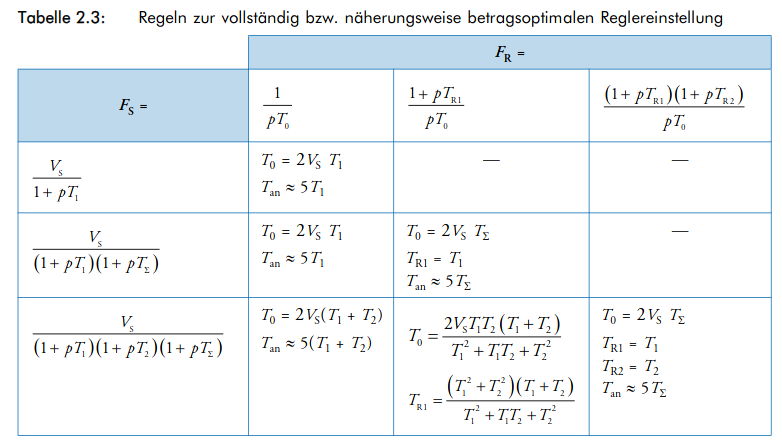
\includegraphics[scale = 0.5]{themen/pict/betragsoptimal.png}

\subsubsection{Symmetrisches Optimum, Einstellregel nach Kessler}


\begin{minipage}{0.45\textwidth}
  Einstellregeln PI-Regler:\\
  \mainformular{$ T_R = 4 T_{\Sigma}$ ; \\
  $ T_0 = 2V_S \frac{T_{\Sigma}T_R}{T_S} = 8V_S\frac{T_{\Sigma}^2}{T_s}$ }\\
  Einstellregel PID-Regler:\\
  \mainformular{$F_R= \frac{(1+pT_R)^2}{pT_0}$ ; \\
  $T_R = 8 T_{\Sigma}$ ; \\
  $T_0 = \frac{128T_{\Sigma}^3 V_S}{T_2T_3}$}
\end{minipage}
\begin{minipage}{0.45\textwidth}

\legende{
Anwendung in elektrischer Antriebstechnik
}
\end{minipage}


\subsubsection{Stochastisches Optimum}

\begin{minipage}{0.45\textwidth}
  \mainformular{$T_R = T_S$; $T_0 = \frac{1}{2} V_S T_{\Sigma}$}\\
  $\omega_d = \frac{\sqrt{2}}{T_{\Sigma}}$; $ \gamma = 35^\circ$

  Mit zusätzlichem Verzögerungsglied wird Führungsverhalten verbessert (weniger Überschwingen)\\
  $F_V(p) = \frac{1}{1+pT_V} $ \\
  mit $T_{VStO} = 1,2 T_{\Sigma}$
\end{minipage}
\begin{minipage}{0.45\textwidth}
\legende{
Verbesserung des Störverhaltens\\
Erhöhung der Reglergeschwindigkeit
}
\end{minipage}


\subsubsection{Einstellregel nach Naslin}
\begin{minipage}{0.45\textwidth}
Sei $F_w(p) = \frac{b_0}{a_0+a_1p+a_2p^2} = \frac{\frac{b_0}{a_0}}{1+\frac{a_1}{a_0}p+\frac{a_2}{a_0}p^2}$

Übertragungsfunktion des Schwingungsglieds: \\
$F_s(p)= \frac{1}{1+p2DT_0 + p^2T_0^2}$

Koeffizientenvergleich:
$4D^2 = \frac{a_1^2}{a_0a_2}$

und allg:
$\alpha = \frac{a_i^2}{a_{i-1} a_{i+1}}$


\end{minipage}
\begin{minipage}{0.45\textwidth}
\legende{
anwendbar, wenn Übertragungsfunktion\\ der Strecke bekannt\\
günstiges Führungsverhalten aber ohne\\ kurze Ausregelzeiten\\
nur für Zählerpolynom nullter Ordnung\\ und geradzahliges Nennenpolynom
}
\legende{günstige Verhältnisse: $1,5 \leq \alpha \leq 2,5$}
\end{minipage}


\end{document}
